\documentclass[USenglish,oneside,twocolumn]{article}

\usepackage{etex}
\usepackage[big]{dgruyter_NEW}
\usepackage[justification=centering]{caption}
\usepackage[justification=centering]{subcaption}
\captionsetup{compatibility=false}
\usepackage[ruled,algosection,noend,linesnumbered]{algorithm2e}
\usepackage{adjustbox}
\usepackage{mathtools}
\DeclarePairedDelimiter{\ceil}{\lceil}{\rceil}
\usepackage{amsfonts}
\usepackage{stmaryrd}
\usepackage{amsmath}
\usepackage{amssymb}
\usepackage{amsthm}
\usepackage{color}
\usepackage{float}

\usepackage{tikz}
\usetikzlibrary{shapes, positioning, matrix, backgrounds}

\newtheorem{privdef}{Privacy Definition}
\newtheorem*{secgme}{Security Game}
\newtheorem{secthm}{Security Theorem}
\newtheorem{seccjt}{Security Conjecture}
\newtheorem{seclem}{Security Lemma}
\newtheorem{lemma}{Lemma}
\newtheorem{theorem}{Theorem}


\newenvironment{subproof}[1][\proofname]{%
  \renewcommand{\qedsymbol}{$\blacksquare$}%
  \begin{proof}[#1]%
}{%
  \end{proof}%
}

\newcommand{\todo}[1]{\textcolor{red}{TODO: #1}}
\newcommand{\raphael}[1]{\textcolor{blue}{Raphael: #1}}
\newcommand{\george}[1]{\textcolor{green}{George: #1}}

\cclogo{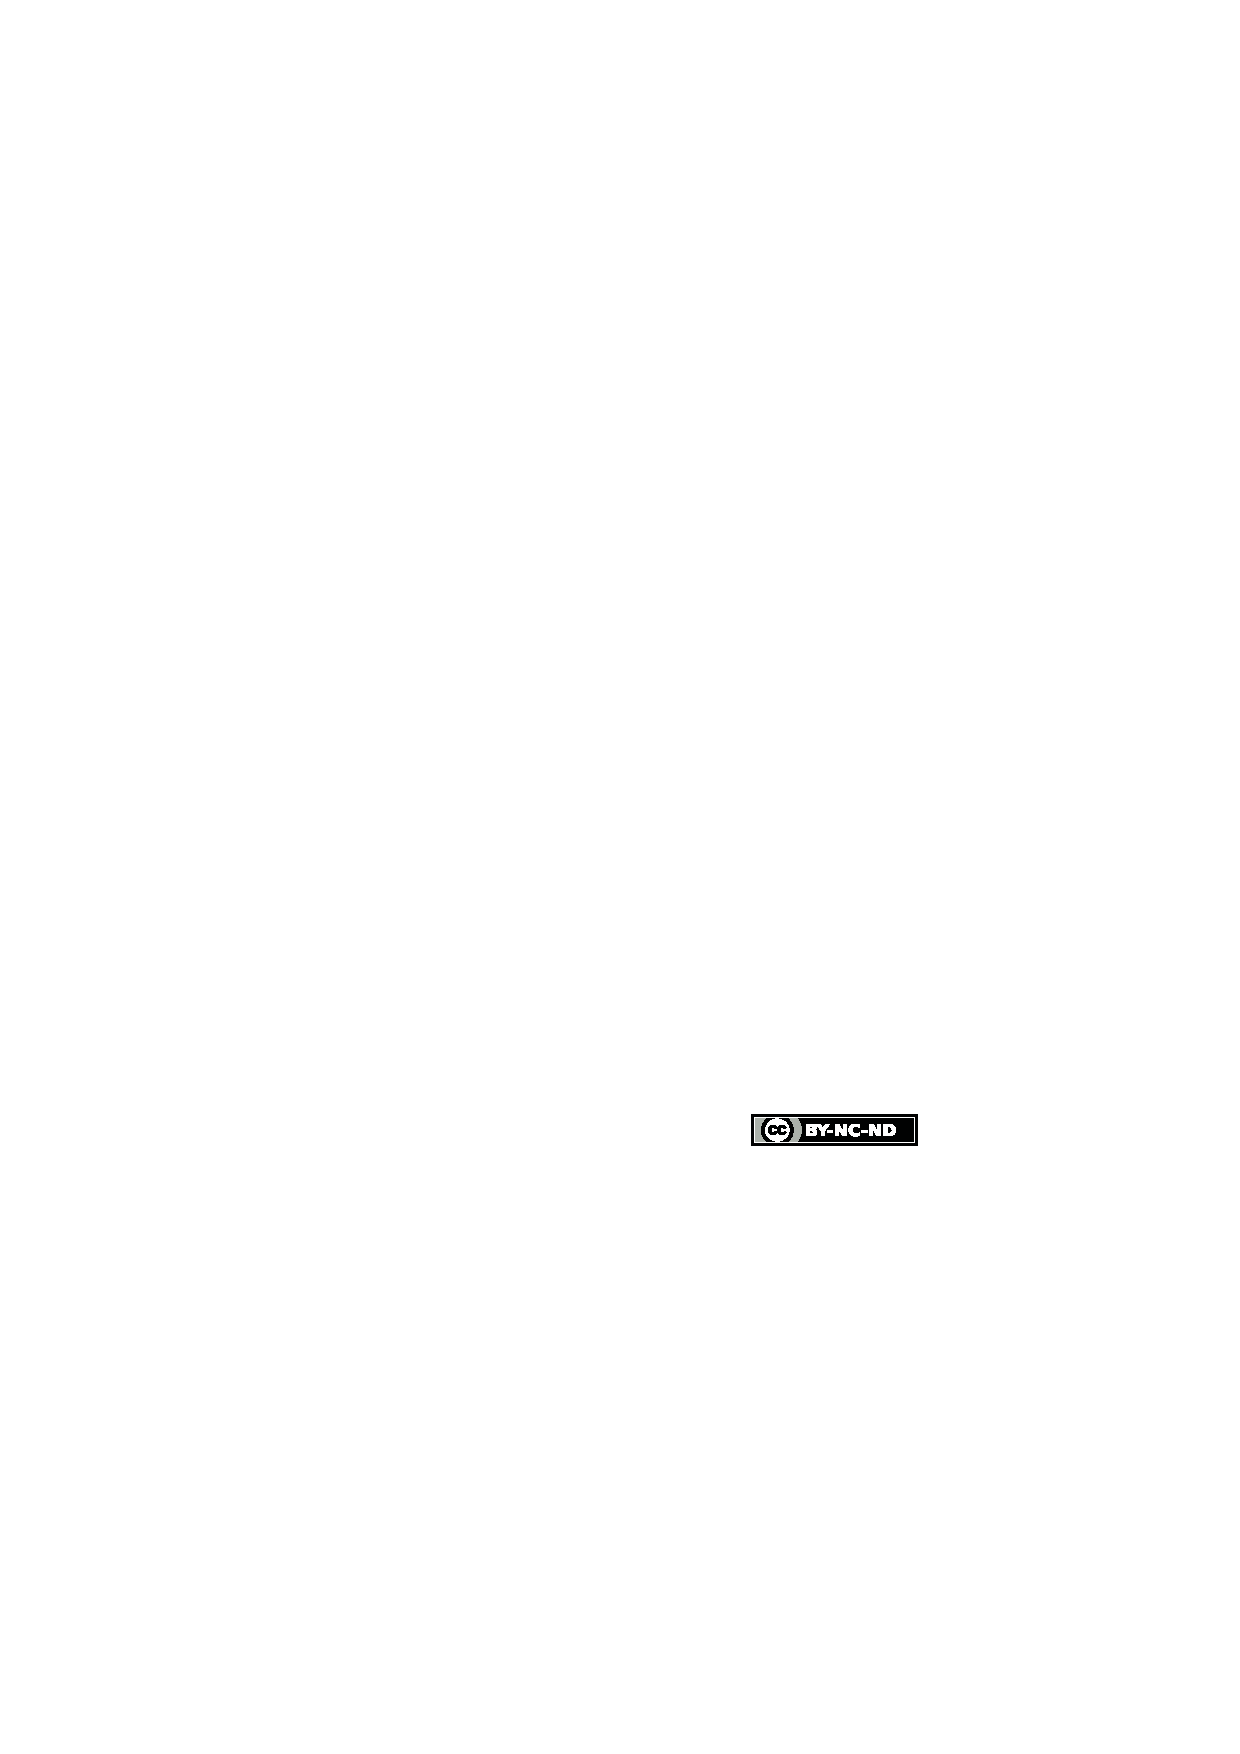
\includegraphics{by-nc-nd.pdf}}
  
\begin{document}
 
\author[1]{Raphael R. Toledo}

\author[2]{George Danezis}

\affil[1]{University College London (r.toledo@cs.ucl.ac.uk)}

\affil[2]{University College London (g.danezis@ucl.ac.uk)}

  \title{Mix-ORAM: Using delegated shuffles.}

  \begin{abstract}
{
Oblivious RAM is a key technology for securely storing data on untrusted storage but is commonly considered impractical due to its high overhead. Indeed, to ensure full privacy to the user, the database has to be periodically randomized, i.e. re-encrypted and shuffled, by the client. To attain full privacy, the computation and communication costs the client incurs are in reality super linear in the number of records, this very price deters the use of ORAM for most applications. We propose in this paper to increase ORAM's appeal by delegating the randomization process to semi-trusted third parties such that the clients are oblivious to the corresponding overhead. To do so, we present four different designs inspired by mix-net technologies and evaluate them. Results results results
}
\end{abstract}
  \keywords{Oblivious RAM, Mix-net, Private Queries}
%  \classification[PACS]{}
%  \communicated{...}
%  \dedication{...}

\journalname{Proceedings on Privacy Enhancing Technologies}
%\DOI{10.1515/popets-2016-0035}
%\startpage{1}
%\received{2016-02-29}
%\revised{2016-06-02}
%\accepted{2016-06-02}

%\journalyear{2016}
%\journalvolume{2016}
%\journalissue{4}

\maketitle
%
\section{Introduction}\label{Introduction}
%

Cloud technologies offer the ability to save impressive amounts of data safely and privately on remote servers. To do so, not only the data integrity must be preserved but also the confidentiality of the data content and meta data from both external adversaries and the cloud itself.
Cryptographic measures are thereby taken such as secure communication channels, user authentication, data encryption and integrity checking.
These actions, however, do not prevent the leakage of all meta data: the server owner can monitor user activities and watch which records were fetched. \\


Oblivious RAM (ORAM)~\cite{goldreich87}, or Oblivious Storage (OS)~\cite{boneh2011}, precisely prevents an adversary from observing the record access, and do so by introducing a pairing of virtual and real, or remote and local, indices. In these schemes, the records are encrypted and permuted before being uploaded to the untrusted storage and the information to decrypt the records,the encryption keys, and make the matching between the remote and local indices, a pseudo random generator seed for instance, is saved locally. When the user seeks a given record, the local client computes with the seed the corresponding remote index, fetches the encrypted data block obliviously and decrypts it. After a number of accesses, in order to render any leaked information obsolete, the database is fetched and before being uploaded back to the remote server, encrypted and shuffled once again during a so called eviction process before.

This randomization is the main bottleneck of ORAM. Indeed, we assume in such design that the number of records stored remotely is orders of magnitude higher than the client storage. As every record must be re-encrypted and permuted locally to ensure nothing is leaked, the client has to download and process the database by chunks, and do so several times to undeniably hide from the adversary the records' ordering. Thus as the the database size grows, the randomization cost rises super linearly.\\

Mix networks~\cite{chaum1981untraceable} are a solution widely applied in anonymity systems to obliviously shuffle packets. A batch of packets is processed by the mix-net in that each mix re-encrypts, or decrypts, and shuffles the packets before sending them to the next mix. For the adversary to link the mix-net's input and output, all of the mixes used in the shuffling have to be compromised.
As the mixes perform all the operations needed in ORAM, mix-nets inspired designs could thus address the delegation of ORAM's randomization process but at high price since the used of several mixes is needed to ensure the confidentiality of the randomization and that the computation and communication costs are linear in the number of mixes. If using these designs, methods to amortize the eviction must be taken into account to make the randomization practical.\\

In this work, we present several distributed systems' designs inspired by mix-nets to safely delegate ORAM's randomization process to semi-trusted third parties.
The advantages of such practices are, besides the reduction of the client computation, the possibility to delay the eviction to quieter times, the database availability during the eviction process regardless of the ORAM design and the independence from centralized parties.

Our contributions are listed as following:

\begin{itemize}
 \item We present and motivate the use of mix-net with ORAM.
 \item We present a number of designs, improve them with load balancing via parallel mixing and compare their costs and efficiency.
 \item We introduce a new security definition of ORAM's eviction. %indistiguishability between accessed and unretrieved elements
\end{itemize}

We present the related work, the ORAM model, its associated threat model and explaining the different costs in Section~\ref{Related} and~\ref{Prelim}, we use random transposition shuffles them in ORAM and together with a mixnet and discuss various optimizations in Section~\ref{Mix-ORAM}. We then present our implementation and compare the costs with several designs in Section~\ref{Evaluation}.
We finally evaluate our schemes and discuss about the advantages and drawbacks of using mix-nets.
%

\section{Related Work}\label{Related}
\noindent\textbf{ORAM.}
ORAM technologies were first presented by Goldreich and Ostrovsky in 1990~\cite{ostrovsky1990efficient} to prevent reverse engineering and protect softwares run on shielded CPU, the concept was update in 2011 with Oblivious Storage (OS)~\cite{boneh2011} in the context of untrusted remote storage.
Since then, several types of enhancement have been proposed including \textit{data structures} diversification~\cite{goldreich1996software,stefanov2011towards,stefanov2013path,ren2014ring} with trees, partitions and hierarchichal solutions appearing,
the use of more and more sophisticated \textit{security definitions} with statistical security~\cite{damgaard2011perfectly,ajtai2010oblivious} and differential privacy~\cite{wagh2016root}, and the revision of \textit{item lookups} with cuckoo hashing~\cite{pinkas2010oblivious} and bloom filters~\cite{williams2008building}.
Most ORAM constructions are based on a single client-server model, but multi-user designs were gradually introduced as \cite{backesanonymous} in 2016 which also provides user anonymity, some relying on access control~\cite{franz2011oblivious} or group access~\cite{goodrich2012privacy}.
The eviction process is one of the principal problems of ORAM, the clients have to re-encrypt and process the whole database for extensive period of time during which record access is usually not possible, some designs permitting read while shuffling as \cite{boneh2011}.\\

\noindent\textbf{Shuffling and Sorting.}
Shuffle and sorting algorithms are a thoroughly researched subject central to ORAM for the randomization process. However most of the existing methods are not useful for ORAM as they are not oblivious -in that the permutations done depends on the data itself-.

Examples of oblivious sorting algorithms include sorting networks such as Batcher's~\cite{batcher1968sorting} and the ones based on AKS~\cite{ajtai19830} which unfortunately were proved to be impractical because of the high number of I/Os, Batchers using $\mathcal{O}\left ( n \log n \right)$ I/Os and AKS having a high constant factor, but also more recent and efficient ones~\cite{paterson1990improved}.
The randomized Shellsort~\cite{goodrich2010randomized} is an elegant simple data-oblivious version of the Shellsort algorithm running in $\mathcal{O}\left ( n \log n \right)$ time that sort with high probability.
The Zig Zag sort~\cite{goodrich2014zig}, presented in 2014, is the deterministic data-oblivious variant of the Shellsort with running time of $\mathcal{O}\left ( n \log n\right)$.
Lastly, the bucket sort Algorithm was both studied in Melbourne shuffle~\cite{ohrimenko2014melbourne} where a user rely on temporary arrays and dummies and in~\cite{goodrich2012anonymous} with the use of a parallel mixnet.\\

\noindent\textbf{Mix-nets.}
Mix-nets were first presented for anonymous e-mailing by David Chaum in 1981~\cite{chaum1981untraceable}. As they became popular many improvements were made over the years~\cite{moller2003mixmaster,danezis2003mixminion,danezis2004minx,danezis2009sphinx}. Mix-nets' main goal is to give users some anonymity by hiding the correspondence between the incoming users' packets and the mix-nets output. To do so, the users' packets go through several mixes which permute them and refresh their encryption. Either reencryption~\cite{wikstrom2006adaptively} and onion encryption can be used, proofs of shuffle~\cite{groth2007verifiable,groth2007non,bayer2012efficient} and Randomized Partial Checking~\cite{jakobsson2002making} can help verify the shuffle correctness.

This work is inspired by the mix-net technology for its encryption and permutation functionalities, however, only the packet unlinkability property is of interest for ORAM as the packets come from a single user.
%
\section{Preliminaries}\label{Prelim}
%
\subsection{Model}\label{Model}

ORAM systems actually rely on two types of data arrays. One we call database and comprises the user's encrypted records and some dummies and the other one we call cache, e.g. the shelter in~\cite{goldreich87}, of lesser size and used to store the fetched records in order to hide the number of times they were accessed.\\

\noindent\textbf{Access method:} The client first downloads the cache and checks whether the desired record is present, if so a dummy is fetched from the database else the desired record. Finally, the fetched element is encrypted and updated in the cache which is sent back to the ORAM.\\

\noindent\textbf{Eviction method:} When the cache is full, the client empties it by starting the eviction process. To do so, the client first \textit{rebuilds} the database by merging obliviously the cache and the database and afterwards, starts the \textit{oblivious shuffle}.

\noindent The rebuild phase consists in placing obliviously records from the cache back to the ORAM database. The client begins by downloading the cache, then re-encrypts the records and discards any dummies contained within it. It next fetches all the records previously accessed from the database, and overwrites them one by one with their cached version or with a dummy before updating them back in the database. The cache is now empty.

\noindent The client starts the oblivious shuffle by selecting a set of mixes from the mix-net and sending to them randomization instructions containing the list of participating mixes and the seeds used for shuffling and encrypting. When receiving the records, the first mixes fetch the database, encrypt the records, shuffle and transmit them to the next mixes according to these instructions.\\

We consider here an ORAM remote server consisting of a database with memory of $n\ b$-bit long data blocks and a cache with memory of $s,\ s\ll n,\ b$-bit long data blocks. We furthermore consider a mix-net composed of $m$ mixes with memory of $n/m$ data blocks, and a client with memory of $s$ data blocks. The ORAM server, the mixes and the client additionally have a small memory of capacity $\mathcal{O}(m)$ to store extra information about permutation and encryption.

\subsection{Security definitions and Threat model}\label{Threat}

We presume here of the existence of motivated adversaries trying to subvert a target user's privacy and perhaps compromise his data integrity. We assume the target user utilizes an ORAM system, compliant with the Privacy Definition~\ref{def:Oram} introduced by Stefanov et al.~\cite{stefanov2011towards}, to protect his data.
We futhermore assume that all communication between the client, ORAM server and mixes may be intercepted as in the \textit{global passive adversary} assumption however only message timing, volume and size from honest parties can be known thanks to packet encryption.
Finally, we suppose the adversaries have corrupted a number of machines to achieve their goal, unless said otherwise, the ORAM server and all but one mix are considered compromised. We will assume that the compromised machines behave in a \textit{honest but curious} way in that every operation is correctly performed but passively recorded and shared with the adversaries.

\begin{privdef}\label{def:Oram}
Let's denote a sequence of $k$ queries $\text{seq}_k=\{(\text{op}_1, \text{ad}_1, \text{data}_1), \text{ ...},(\text{op}_k, \text{ad}_k, \text{data}_k)\}$, where $op$ denotes a read or write operation, $ad$ the address where to process the operation and $data$ the block to write if needs be else $\perp$.
We denote by $ORAM(seq_k)$ the resulting randomized data access from the ORAM process with input $seq_k$.
The ORAM guarantees that $ORAM(seq_k)$ and $ORAM(seq'_{k'})$ are computationally indistinguishable if their lengths are equal ($k=k'$).
\end{privdef}

This work focuses on the ORAM eviction process and more precisely on the randomization phase where sequences of data-blocks are shuffled in an oblivious manner in order to hide the records indexes after access information has leaked. For instance, in the Square Root solution~\cite{ostrovsky1990efficient} the problem refers to the eviction of the shelter in the database and the upper partitions in a lower one in the Hierarchical case~\cite{goldreich1996software}. We evaluate our designs with the following Security Game and consider the adversaries have won the game when discovering the ordering of the remote records.

%
\begin{secgme}
An adversary gives to the user two ORAM query sequences $\text{seq}_k$ and $\text{seq}_k'$ of the same size. The user chooses randomly one of the two, executes it and start the eviction. At the end of the eviction the adversary picks which ORAM query sequence was chosen. The adversary wins if the right sequence is chosen with probability higher than $\Pr = \frac{1}{2}+\epsilon$, with $\epsilon\ll\frac{1}{2}$.
\label{def:Game}
\end{secgme} 
%

\noindent\textbf{Costs.} We denote the communication costs by $\omega$ for the number of \emph{bits} sent by the ORAM, $\gamma$ by the client, and by $\mu$ sent per mix. 
We classify the computation cost under its function (encryption, shuffle and secret generation), and the machine doing the computation. 
%
\subsection{Cryptographic Primitives}
\noindent\textbf{PRG \& Seeds.}
ORAM systems make use of pseudo random generators (PRG) and seeds to save the matching between remote and real indices. A distribution $\mathcal{D}$ over strings of length $l$ is said pseudo random if $\mathcal{D}$ is indistinguishable from the uniform distribution over strings of length $l$~\cite{katz2014introduction}. That means it is infeasible for any polynomial-time adversary to tell whether the string was sampled accordingly to $D$ or was chosen uniformly at random. A PRG is a deterministic algorithm that receives as an input a short random seed and stretches it into a long pseudo random stream.\\\

\noindent\textbf{Encryption.}
ORAM designs heavily rely on encryption mechanism to obfuscate the database records as the records must be re-encrypted during the eviction and access processes.

Advanced Encryption Standard (AES)~\cite{daemen2013design} was conceived for high speed and low RAM requirements. It can present throughput over 700 MB/s per thread on recent CPUs such as the Intel Core i3~\cite{mcwilliams2014hardware} which makes it the ideal choice for ORAM.

To minimize the size of the instructions stored and sent by the client, we make use of elements of a cyclic group of prime order satisfying the decisional Diffie-Hellman assumption. The mixes make use of these elements and derive the different permutation seeds and encryption keys with the a key derivation function, such as the HKDF~\cite{XXXHKDF}, and refresh the them at each round by blinding them with the shared secrets as in \cite{danezis2009sphinx}. 
%
\section{Mix-ORAM}\label{Mix-ORAM}
In this section, we first introduce the different encryption methods we will use to encrypt the records during the eviction. We then present a simple but impractical Mix-ORAM case before optimizing it with the use of distributed shuffle algorithms. 
%
\subsection{Mix and User encryption methods}\label{Enc}
We present in this work different ways to delegate the eviction process to a semi-trusted mix-net proposing two re-encryption methods. For each method, we show how the mix-nets encrypt the records and how the client recovers a record plain text.
We make the assumption that all data has first been encrypted by the user before using the ORAM. \\

\textbf{Layered method.} In the Layered method, we use the data structure shown in Table~\ref{ldata} composed of an IV token, and a label appended to the record, e.g. the record real indices. The underlying principle of the layered method is to let the mixes encrypt the records with AES in CBC mode thanks to IV tokens during the eviction and to let the client decrypts the requested records after the access. To maintain a low number of encryption layers on top of the records, we propose to modify the access method to fetch more records from the database.

\begin{table}[H]
\begin{minipage}[t][][b]{.475\textwidth}
\vspace{0pt}
\centering
\begin{tabular}{|c|c|}
IV token  &  data = label | record  \\
$8\cdot\ceil{\log(n)/8}$ bit  &  $8\cdot\ceil{\log(n)/8}+b$ bit   \\
\end{tabular}
\centering
\caption{Layered method data structure.}
\label{ldata}
\end{minipage}
\end{table}

During the eviction, the mixes use the IV token as seed to generate an initialisation array. AES-CBC is then used to encrypt the data with the IV and the secrets shared with the client. The $8\cdot\ceil{\log(n)/8}+b$ first bit of the data is then used as a seed to generate an IV with which the IV token is encrypted under AES-CBC and with the shared secrets. Once all elements haven been re-encrypted, they are forwarded to the next mixes.

To decrypt a record, the client make uses of the trial error process written in Algorithm~\ref{alg:ldec}. Using the shared secrets, the IV token is first deciphered then the data, these two operations are repeated $r$ times in total. The client then uses its own secret key to decipher the IV and the data another time, if the label is the right one, the process stops, if not the client cancels the last decryption and starts again.
To encrypt a record, the client generates the IV token and label, encrypts the data with its own secret key and the IV produced from the IV token, and encrypts the IV with its own secret key and an IV produced from the data.
 
As the number of encryption layers per record may vary, we delay the decryption of the fetched record to avoid a timing attack. When retrieving a record, before sending the cache back to the ORAM server, the client encrypts the retrieved record with its own key and updates it back in the cache before uploading the latter.
After doing so, the client locally decrypts the previous encryption and starts the decryption method described above. Once the plain text is recovered, a new IV token is generated, the label is appended to the record, the data is encrypted with the IV produced from the IV token and the private key. The next time the cache is fetched, the cached version of the record is overwritten with the new version. 

We now look at the average number of encryption layers a record has before being decripted. Making the assumption that the record access distribution is uniform, we can represent the problem of accessing all records at least once as a coupon collector problem. In that case, we expect $E[e]\leq(n/s)\cdot H_n )$ evictions before all records have been fetched once with $H_n$ the $n^{th}$ harmonic number, and the expected number of layers per card is $E[r]\leq{r/s} \cdot \left ( \frac{n+1}{2}\cdot(H_n-1/2)+1/2 \right )$. For $n=10^6$ and $s=\sqrt{n}$, we have $E[e]\approx 15 \cdot 10^3$ and $E[r]\approx 7\cdot 10^3 \cdot r$.
\begin{proof}
Lets $\tau_n$ be the random number of coupons collected when the first set contains every $n$ types. We have, $E[\tau_n]=n\sum_{i=1}^n \frac{1}{i} = n \cdot H_n$.
Since we fetch $s$ unique records per eviction (we cannot fetch a record already in the stash), the previous result is an upper bound of the number of requests needed and so the expected number of eviction is $E[e]\leq n/s\ H_n$.

We now want to find the average number of encryption layers per record before decryption, this is equivalent to finding the average number of evictions before a record is deciphered. 
Hence we have, $E[r]\leq r/s \cdot \sum_{i=1}^n E[\tau_i] = r/s\ \sum_{i=1}^n \left (\frac{(n+1-i)(n+i)}{2}\cdot \frac{1}{i}\right )$ from which can be calculated the result presented earlier. 
\end{proof}

To reduce these numbers, we modify the access method as written in Algorithm~\ref{alg:lacc}. When the client requests a record from the database, $d$ other records are chosen uniformly at random from the set of unaccessed records. These records are then fetched, their encryption is refreshed as written previously and the client overwrites with these records their older version on the database. Doing so, choosing a parameter $d$ high enough yields a better approximation of the uniform distribution assumption. We would have thus $E[e]\leq n/(sd) \cdot H_n $ and $E[r] \leq{r/(sd)} \cdot \left [ \frac{n+1}{2}\cdot(H_n-1/2)+1/2 \right ] \ H_n$.
With $d=\sqrt(n)$, we now have $E[e]\leq 15$ and $E[r]\leq 7$.\\

\begin{algorithm}
\SetKwComment{Comment}{//}{}
\DontPrintSemicolon
\KwIn{Record $rec$; \\ \qquad Encryption key $k$; }
$IV \gets urandom(rec.token\cdot k, 128)$;\\
$rec.data \gets enc\left(k,\ IV,\ rec.data \right )$;\\
$IV \gets urandom(rec.data \cdot k, 128)$;\\
$rec.token \gets enc\left(k,\ IV,\ rec.token \right )$;\\
\KwOut{rec}
\caption{Layered encryption primitive}
\label{alg:lencp}
\end{algorithm}

\begin{algorithm}
\SetKwComment{Comment}{//}{}
\DontPrintSemicolon
\KwIn{Record $rec$; \\ \qquad Decryption key $k$; }
$IV \gets urandom(rec.data \cdot k, 128)$;\\
$rec.token \gets dec\left(k,\ IV,\ rec.token \right )$;\\
$IV \gets urandom(rec.token\cdot k, 128)$;\\
$rec.data \gets dec\left(k,\ IV,\ rec.data \right )$;\\
\KwOut{rec}
\caption{Layered decryption primitive}
\label{alg:ldecp}
\end{algorithm}

\begin{algorithm}
\SetKwComment{Comment}{//}{}
\DontPrintSemicolon
\KwIn{Record and index $record,\ index$;  \\ \qquad Shared encryption keys $k_{mix,eviction,round}$;\\ \qquad Private key $prv$;\\ \qquad Number of rounds $r$; \\ \qquad Permutation seeds $\sigma$;}
$j,e=0$;\\
$r\gets decrypt(prv_e,rec)$;\\
\While{$rec.data.label != i$}
{
\If {$e!=0$}
{
$rec \gets encrypt(prv_e,\ rec)$;\\
\ForAll{$k \in \llbracket 1 :r \rrbracket $}
{
	$m\gets retrieve\_mix(\sigma,\ e,\ j,\ index)$;\\
	$rec \gets decrypt(k_{m,\ e,\ j}, rec)$;\\
	$j\gets j-1$;\\
}
}
	$rec \gets decrypt(prv_e,\ rec)$;\\
    $e\gets e-1$;\\
}
\KwOut{rec}
\caption{Layered Decryption algorithm}
\label{alg:ldec}
\end{algorithm}

\begin{algorithm}
\SetKwComment{Comment}{//}{}
\DontPrintSemicolon
\KwIn{ Real record index $index$; \\ \qquad Operation and data $op,\ towrite$; \\ \qquad Encryption keys $k$; \\ \qquad Permutation seeds $\sigma$;\\ \qquad Saved records $recs$;\\ \qquad Number of rounds r;}
$j \gets recover\_index(\sigma, index)$;\\
$cache \gets fetch\_cache()$;\\
\ForAll {$rec \in cache$}
{
$cache[rec]\gets decrypt(k,\ r,\ \sigma,\ cache[rec])$;\\
}
\If{$record \in cache$}
{
$record \gets find(record) $;\\
$tofetch \gets choose\_dummies(cache, d+1)$;\\
}
\Else
{
$tofetch \gets choose\_dummies(cache, d)$;\\
$tofetch \gets tofetch \cup \{j\}$;\\
}
$record,\ d \gets fetch(tofetch)$\\
$update\_cache(recs, encrypt(record))$;\\
$send\_cache()$;\\
\If {$op==read$}
{
$d \gets d \cup \{record\}$;\\
}
\Else
{
$d \gets d \cup \{towrite\}$;\\
}
\ForAll {$rec \in d$}
{
$d[rec] \gets decrypt(k,\ r,\ \sigma,\ d[rec])$;\\
$save(encrypt(k,\ d[rec]))$;\\
}
\KwOut{record}
\caption{Layered access method}
\label{alg:lacc}
\end{algorithm}

\noindent\textbf{Rebuild method.} The rebuild method aims at replacing all the mix encryption layers with new ones in a manner such that the intermediaries never see the  underlying user encryption. In order to achieve this, the encrypted records are first encrypted with the mix encryption keys twice. That way, each mix can either decrypt or re-encrypt the cipher-texts and there will always remain at least one layer of  mix encryption. Contrary to the Layered method, the rebuild method does not rely on a data structure, and the encryption used depends on the records order as we use AES in Counter mode (AES-CTR).

Before sending the records to the untrusted storage, the client encrypts the plain-text thrice. The records are always encrypted with AES in CTR mode and we use as counter the record current index. The first time the record are encrypted with the client own private keys, the second time with the shared secrets of every mix, and finally at the last time the records are permuted with permutation seeds and encrypted with the shared secrets of every mix keys at the same time such that the counters vary.
For the sake of conciseness, we summarize the state of the database with the status $E_{k0}, (\Pi_\sigma, E_{k1})$ that must be understood as the database was first encrypted with the encryption keys $k0$ and then at the same time permuted and encrypted with the permutation seeds $\sigma$ and the encryption keys $k1$.

During the eviction, the mixes first unravel the last layer $(\Pi_\sigma, E_{k1})$ by executing $(\Pi_{\sigma}^{-1}, D_{k1})$. The database is now in the original sequence and encrypted under $E_{k0}$. The mixes then encrypt the records with $E_{k0'}$ before decrypting with $D_{k0}$ thanks to AES CTR commutativity and the invariant counter. The database is now in the original sequence and encrypted under $E_{k0'}$. Finally, the mixes encrypt and permute at the same time the records executing $(\Pi_{\sigma'}, E_{k1})$, the database is now permuted in the random order $\Pi_{\sigma'}$ and encrypted under $E_{k0'}, (\Pi_{\sigma'}, E_{k1'})$. A scheme summarizing the eviction can be seen in Fig.~\ref{fig:AES}.  

\begin{figure}
\begin{minipage}{0.5\textwidth}
\begin{adjustbox}{width=\textwidth}
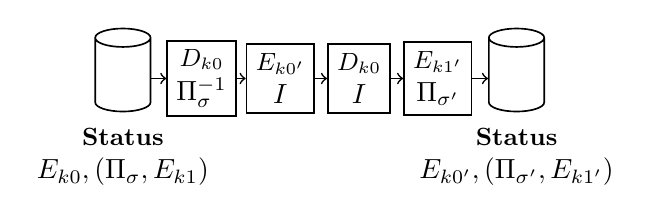
\begin{tikzpicture}[->, auto, semithick]
\tikzstyle{every state}=[fill=white,draw=black,thick,text=black]
\node[draw, cylinder, shape border rotate=90, minimum height=3em,minimum width=2em]    	(X)				  {};
\node[draw=none, align=center] (XX)[below of=X] {\small \textbf{Status}\\$E_{k0}, (\Pi_\sigma, E_{k1})$};
\node[draw, rectangle, align=center]   		(A)[right of=X]   {\small $D_{k0}$\\$\Pi_{\sigma}^{-1}$};
\node[draw, rectangle, align=center]    		(B)[right of=A]   {\small $E_{k0'}$\\$I$};
\node[draw, rectangle, align=center]    		(C)[right of=B]   {\small $D_{k0}$\\$I$};
\node[draw, rectangle, align=center]    		(D)[right of=C]   {\small $E_{k1'}$\\$\Pi_{\sigma'}$};
\node[draw, cylinder, shape border rotate=90, minimum height=3em,minimum width=2em]    	(Y)[right of=D]	  {};
\node[draw=none, align=center] (YY)[below of=Y] {\small \textbf{Status}\\$E_{k0'}, (\Pi_{\sigma'}, E_{k1'})$};
\path
(X.east) edge     	node{}    	(A.west)
(A.east) edge     	node{}    	(B.west)
(B.east) edge     	node{}    	(C.west)
(C.east) edge     	node{}    	(D.west)
(D.east) edge     	node{}    	(Y.west);
\end{tikzpicture}
\end{adjustbox}
\centering
\caption{Eviction under the Rebuild method. \\The first row denotes the encryption (E) and decryptions (D) while the second the permutations ($\Pi$) and $I$ for the identity.} \label{fig:AES}
\end{minipage}
\end{figure}

When retrieving a record, as shown in Alg~\ref{alg:racc}, the client has to compute the record's remote index using the permutation seeds. The client saves all intermediary and final indices and use them as counters to decrypt the record sequentially $r$ times as written in Alg~\ref{alg:rdec}. The client then decrypts the record with all the shared secrets and its own encryption key together with the original index as counter to reveal the plain-text. After updating the cache with the encryption of the record to read or write, the latter is sent back.

\begin{algorithm}
\SetKwComment{Comment}{//}{}
\DontPrintSemicolon
\KwIn{Number of rounds and mixes $r,\ m$; \\ \qquad Encryption keys $k_{mix, round}$; \\ \qquad Mix and Indices $mix,\ round$;}
\ForAll{$i \in \llbracket 1, r\rrbracket$}
{
$record \gets dec(record, k_{mix[r-i],r-i}, ind[r-i] )$;\\
}
\ForAll{$i \in \llbracket 1, m\rrbracket$}
{
$record \gets dec(record, k_{i,0}, index )$;\\
}
\KwOut{record}
\caption{Rebuild decryption algorithm}
\label{alg:rdec}
\end{algorithm}

\begin{algorithm}
\SetKwComment{Comment}{//}{}
\DontPrintSemicolon
\KwIn{Encryption keys $k_{mix,round}$; \\ \qquad Permutation seeds $\sigma$; \\ \qquad Record and index $record,\ index$;  \\ \qquad Operation and data $op,\ towrite$;  \\ \qquad Number of rounds and mixes $r,\ m$;}
$indices \gets \{\}$;\\
$mix\gets \{\}$;\\
\ForAll{$i \in \llbracket 1, r\rrbracket$}
{
$mix,\ indices \gets recover\_indices(index,\ r,\ \sigma)$;\\
}
$cache \gets fetch\_cache()$;\\
\If{$record \in cache$}
{
$record \gets find(record)$;\\
$tofetch \gets choose\_dummies(cache, 1)$;\\
}
\Else
{
$tofetch \gets indices[r]$;\\
}
$record, d \gets fetch(tofetch)$;\\
$record \gets decrypt(record,k,\sigma)$;\\
\If {$op==read$}
{
$update\_cache(encrypt(record,k,\sigma))$;\\
}
\Else
{
$update\_cache(encrypt(towrite,k,\sigma))$;\\
}
$send\_cache()$;\\
\KwOut{record}
\caption{Renovating access method}
\label{alg:racc}
\end{algorithm}

%
\subsection{A simple Mix-ORAM}\label{SMO}
%
We consider here the mix-net in a classic cascade configuration as depicted in Fig~\ref{fig:CascadeArch} and present two designs with either the use of the layered encryption method or the rebuild method. We also want to remind that we consider the database to always be permuted according to a number of seeds, denoted $\Pi_{\sigma}$, the eviction goal being to obviously sort the database to a new state $\Pi_{\sigma'}$.

During the eviction process, the whole database makes a round trip through the mix-net before being updated back to the database. During the way in, the mixes cancel the previous permutation the database has incurred thanks to the old seeds $\sigma$ given by the client. While during the way out, the mixes permute the database according to the new ones $\sigma$ as shown in Alg~\ref{alg:CSort}. At the end of the eviction, or after verification if any, the old seeds are overwritten with the new ones.

When retrieving a record, the user recovers the remote index thanks to the last used seeds. We wrote in Algorithm~\ref{alg:CIL} a method to compute all intermediary indices and mixes, the last index being the one sought.

\begin{figure} \label{CascadeArch}
\centering
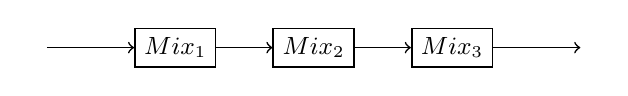
\begin{tikzpicture}[->, auto, semithick, node distance = 5em]
\tikzstyle{every state}=[fill=white,draw=black,thick,text=black]

\node[draw=none, rectangle]    		(X)   {};
\node[draw, rectangle]   		(A)[right of=X]   {\small $Mix_{1}$};
\node[draw, rectangle]    		(B)[right of=A]   {\small $Mix_2$};
\node[draw, rectangle]    		(C)[right of=B]   {\small $Mix_3$};
\node[draw=none, rectangle]    		(Y)[right of=C]   {};

\path
(X.east) edge     	node{}    	(A.west)
(A.east) edge     	node{}    	(B.west)
(B.east) edge     	node{}    	(C.west)
(C.east) edge     	node{}    	(Y.west);

\end{tikzpicture}
\caption{Cascade architecture with three mixes.}
\label{fig:CascadeArch}
\end{figure}

\begin{algorithm}
\SetKwComment{Comment}{//}{}
\DontPrintSemicolon
\KwIn{Old and new private seed $\sigma_i,\ \sigma_i'$;\\ \qquad Data $data$;}
\If {in}
{
$data \gets \Pi^{-1}_{\sigma_i}\left ( data \right )$;\\
}
\Else
{
$data \gets \Pi_{\sigma_i'}\left ( data \right )$;\\
}
\KwOut{$data$}
\caption{Cascade sort for mix $i$}
\label{alg:CSort}
\end{algorithm}

\begin{algorithm}
\SetKwComment{Comment}{//}{}
\DontPrintSemicolon
\KwIn{Seeds $\sigma$;\\ \qquad Number of records and mixes $n,\ m$;\\ \qquad Record index $index$;}
$mixes \gets \{,\}$;\\
$indices \gets \{,\}$;\\
\ForAll {$i \in \llbracket 1, m \rrbracket$}
{
	$index \gets {\Pi}_{\sigma_i}(n,\ index)$;\\
	$mixes \gets mixes \cup \{i\}$;\\
	$indices \gets \cup \{index\}$
}
\KwOut{$mixes,\ indices$}
\caption{Cascade Index Lookup}
\label{alg:CIL}
\end{algorithm}

\noindent\textbf{Layered Cascade.} Before the eviction process starts, the records are in the following state: permuted accordingly to the old seeds $\sigma_i$ and encrypted under the keys $k_i$. The design refreshes the permutation, the database being lastly permuted with $\sigma'$, and add new layers of AES-CBC encryption, the database being encrypted with both $k_i$ and $k_i'$, as shown in Fig~\ref{fig:ASMO_L}.
The first time the database passes through a mix $m_i$, $m_i$ undoes the permutation  inherited from the previous eviction, i.e. $m_i$ performs $\Pi_{\sigma_i}^{-1}\left(DB\right)$ denoted by $\sigma_i$ in the figure. The mix $m_i$ also encrypts the records with the key $k_i$ as detailed before in Algorithm~\ref{alg:lencp}. The second time, the mix $m_i$ performs $\Pi_{\sigma_i'}\left(DB\right)$, and encrypts every record with the new encryption key $k_{i}'$.\\
%
\begin{figure}[H]
\begin{minipage}{0.475\textwidth}
\begin{adjustbox}{width=\textwidth}
\centering
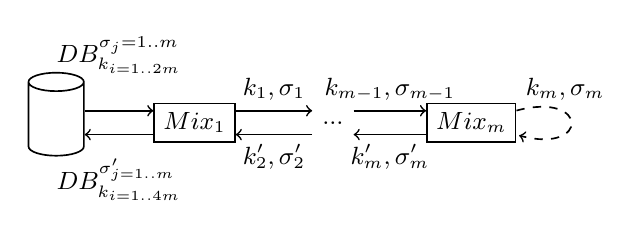
\begin{tikzpicture}[->, auto, semithick,  node distance = 5em]
\tikzstyle{every state}=[fill=white,draw=black,thick,text=black]
\node[draw, cylinder, shape border rotate=90,minimum height=3em,minimum width=2em]    	(0)				  {};	
\node[draw, rectangle]   		(A)[right of=0]   {\small $Mix_{1}$};
\node[draw=none, fill=none]    		(X)[right of=A]   {\small $...$};
\node[draw, rectangle]    		(B)[right of=X]   {\small $Mix_m$};

\path
([yshift=1ex]0.east) edge     	node[above=1em]{\small $DB_{k_{i=1..2m}}^{\sigma_j=1..m}$}    	([yshift=1ex]A.west)
([yshift=-1ex]A.west) edge     	node[below=0.5em]{\small $DB_{k_{i=1..4m}}^{\sigma_{j=1..m}'}$}    	([yshift=-1ex]0.east)

([yshift=1ex]A.east) edge     	node{\small $k_{1},\sigma_1$}    	([yshift=1ex]X.west)
([yshift=-1ex]X.west) edge     	node{\small $k_{2}',\sigma_2'$}    	([yshift=-1ex]A.east)

([yshift=1ex]X.east) edge     	node{\small $k_{m-1},\sigma_{m-1}$}    	([yshift=1ex]B.west)
([yshift=-1ex]B.west) edge     	node{\small $k_{m}',\sigma_{m}'$}    	([yshift=-1ex]X.east)

(B)    edge[loop right, dashed]    node[xshift=-2em,yshift=1.2em]{\small $k_{m},\sigma_{m}$} (B);

\end{tikzpicture}
\end{adjustbox}
\centering
\caption{Layered simple Mix-ORAM eviction.} \label{fig:ASMO_L}
\end{minipage}
\end{figure} 

\noindent\textit{Mix instructions.}
The client sends to every mix three elements of a cyclic group of prime order satisfying the decisional Diffie-Hellman Assumption as in Sphinx~\cite{danezis2009sphinx} $\alpha_{old}$ to undo the old permutations, $\alpha_{new}$ to perform the new ones and  $\beta$ to encrypt the records. Alongside these elements, are sent the signed list of mixes $(ports,\ ips)$ and the database access information $db$ consisting of the IP addresses and access token. The client thus send to each mix $mix_i$:
$$ db,\ \alpha_{i,\ old},\ \alpha_{i,\ new},\ \beta_{i},\ (ports,\ ips) $$

Let $g$ be a generator of the prime-order cyclic group $\mathcal{G}$ satisfying the Diffie-Hillman Assumption and $q$ the prime order of $\mathcal{G}$. We assume that each mix $mix_i$ has a public key $y_i=g^{x_i}\in \mathcal{G}^*$ with $x_i \in_{\mathbb{R}} \mathbb{Z_q}$ alongside the presence of a Public Key Infrastructure to distribute an authenticated list of all $(mix_i, y_i)$.
To generate the $\alpha$s and $\beta$s, the client pick at random in $\mathbb{Z}_q$ for each mix $mix_i$ the elements $z_i$ and $z_i'$. The group elements $\alpha$, $\beta$, shared secrets $sk$ and $ss$ are generated and the encryption keys and permutation seeds are derived as follows:
\begin{align*}
\alpha_i &= g^{z_i},\ sk_i = y_i^{z_i},\ k=hkdf(sk_i)\\
\beta_i &= g^{z_i'},\ s\sigma_i = y_i^{z_i'},\ \sigma=hkdf(ss_i)
\end{align*}

\noindent\textit{Mix operations.} \todo{} \\

\noindent\textit{Costs.}
We have $c_{cmp} = 2\cdot m \cdot n \cdot c_{CBC}$, $c_{client}= x$, $c_{mix}=2\cdot m \cdot n$. The total communication cost is $c_{com}=2\cdot m\cdot n + m\cdot c_{client}$.\\

\noindent\textbf{Rebuild Cascade.} Each of the mixes decrypt and unwrap the records in the first phase then wrap and encrypt in the second, an  blinding phase is added between the two during which the records are only encrypted then decrypted thanks to AES-CTR commutativity as depicted in Fig~\ref{fig:ASMO_CTR}.\\
 %
\begin{figure}[H]
\begin{minipage}{0.475\textwidth}g
\begin{adjustbox}{width=\textwidth}
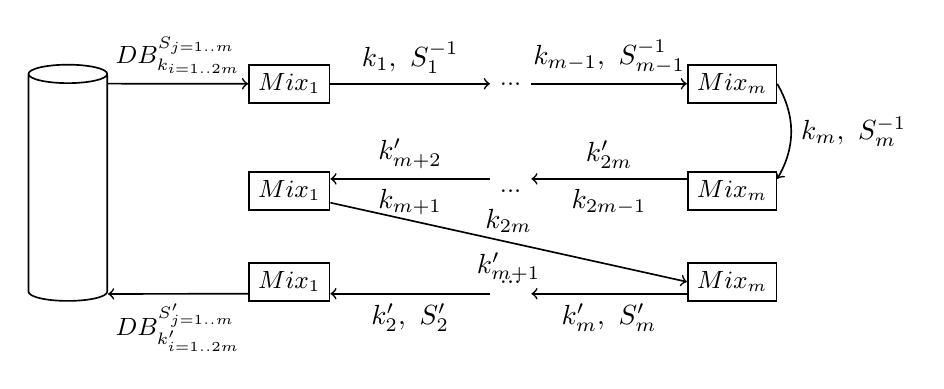
\begin{tikzpicture}[->, auto, semithick, node distance = 8em, every loop/.style={<-}]
\tikzstyle{every state}=[fill=white,draw=black,thick,text=black]


\node[draw, cylinder, shape border rotate=90,minimum height=3cm,minimum width=1cm, anchor=west]    	(0)				  {};	
\node[draw, rectangle]   		(A)[right =of 0.north, anchor = north]   {\small $Mix_{1}$};
\node[draw, rectangle] (A')[right of=0]{\small $Mix_{1}$};
\node[draw, rectangle]   		(A'')[right=of 0.south, anchor = south]   {\small $Mix_{1}$};

\node[draw=none, fill=none]    		(X)[right of=A]   {\small $...$};
\node[draw=none, fill=none]    		(X')[right of=A']   {\small $...$};
\node[draw=none, fill=none]    		(X'')[right of=A'']   {\small $...$};

\node[draw, rectangle]    		(B)[right of= X]   {\small $Mix_m$};
\node[draw, rectangle]    		(B')[right of=X']   {\small $Mix_{m}$};
\node[draw, rectangle]    		(B'')[right of= X'']   {\small $Mix_m$};

\path 
([yshift=0.85cm]0.north east) edge     	node{\small $DB_{k_{i=1..2m}}^{S_{j=1..m}}$}    	(A.west)

(A.east) edge node{$k_{1},\ S_{1}^{-1}$}    	(X.west)

(X.east) edge node{$k_{m-1},\ S_{m-1}^{-1}$}    	(B.west)

(B.east) edge[bend left] node{$k_{m},\ S_{m}^{-1}$} ([yshift=1ex]B'.east)

([yshift=1ex]B'.west) edge[align=center] node[above]{$k_{2m}'$} node[below]{$k_{2m-1}$}    	([yshift=1ex]X'.east)

([yshift=1ex]X'.west) edge[align=center] node[above]{$k_{m+2}'$} node[below]{$k_{m+1}$}    	([yshift=1ex]A'.east)

([yshift=-1ex]A'.east) edge[align=center] node[above]{$k_{2m}$} node[below]{$k_{m+1}'$} (B''.west)

([yshift=-1ex]B''.west) edge    node{$k_{m}',\ S_{m}'$}  ([yshift=-1ex]X''.east)

([yshift=-1ex]X''.west) edge    node{$k_{2}',\ S_{2}'$}  ([yshift=-1ex]A''.east)

([yshift=-1ex]A''.west) edge node{\small $DB_{k_{i=1..2m}'}^{S_{j=1..m}'}$} ([yshift=-0.8cm]0.south east);


\end{tikzpicture}
\end{adjustbox}
\centering
\caption{Renovating a simple Mix-ORAM.} \label{fig:ASMO_CTR}
\end{minipage}
\end{figure} 
%
\noindent\textbf{Message Format.}
We derive the keys and seeds as previously however we produce twice more shared keys than usual for the wrapping and unwrapping phases. \iffalse\\
Let $\kappa$ be the security parameter. We call $\mathcal{G}$ a prime order cyclic group satisfying the Decisional Diffie-Hellman Assumption. $\mathcal{G}^*$ is the set of non-identity elements of $\mathcal{G}$. The element $g$ is a generator of the group, and $q$ is the prime order of $\mathcal{G}$ with $q \approx 2^{2\kappa}$.\\
We suppose each mix owns a pair of keys ($\ priv_i \in \mathbb{Z}_{q}^*$, $pub_i=g^{priv_i}\in \mathcal{G}^*$). We assume the existence of a PKI that publishes a list of all ($mix_i$,\ $pub_i$) pair.
The client randomly chooses $x\in_\mathcal{R} \mathbb{Z}_q^*$ and sends to the mix $mix_i$ the element $\alpha_i=g^{x\cdot b_i}$ with $b_i$ a binding factors, the shared secret is then $s_i=pub_i^{x\cdot b_i}$.
\fi
The client only need to send to the mixnet session keys to access the database $(id,\ token)$, the client secrets used to compute the shared secret $( \alpha_{i,old},\ \alpha_{i,new} )$, and the signed next mix addresses $(ports,ips)_{signed}$.
The message format is then: $$E_{pub,\ mix_i}\left(id,\ token,\ \alpha_{i,old},\ \alpha_{i,new},\ (ports,\ ips)_{signed} \right)$$ 


\noindent\textbf{Costs.} For 128-bit security, group elements can be expressed in just 32 bytes. We have $c_{cmp} = 3 \cdot m \cdot n \cdot c_{CTR} $, $c_{client}=  x$, $c_{mix}=3n$. The total communication cost is $c_{com}=3 \ cdot m \cdot n + c_{client}$.\\


These schemes are not efficient as instead of re-encrypting each record twice as in the Melbourne Shuffle, at least $2\cdot m$ encryption per element are necessary to achieve perfect security. The whole database also goes through every node twice which incur severe delays. To increase the mix-net efficiency, we study in the following sectin parallelization to distributing the workload among mixes.
% 
\subsection{Parallelizing the Eviction process.}\label{Parallel}
In this section, we replace the cascade configuration of the mix-net with a parallel one as depicted in Fig~\ref{fig:mix_par} and use random transposition shuffles (RTS) to model the parallelization. We also calculate the number of rounds needed to reach perfect security by presenting firstly the mixing time of $k$-RTS before introducing ORAM assumptions to reduce the expected time to achieve randomness.

Parallel mix-net ...

\begin{figure}
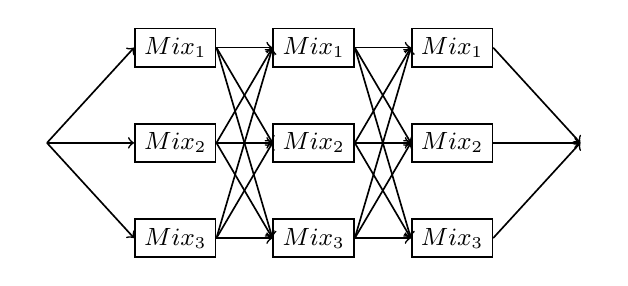
\begin{tikzpicture}[->, auto, semithick,  node distance = 5em]
\tikzstyle{every state}=[fill=white,draw=black,thick,text=black]

\node[draw=none, fill=none]    		(X)   {};
\node[draw, rectangle]    		(B)[right of=X]   {\small $Mix_2$};
\node[draw, rectangle]   		(A)[above=2em of B]   {\small $Mix_{1}$};
\node[draw, rectangle]    		(C)[below=2em of B]   {\small $Mix_3$};
\node[draw, rectangle]   		(A')[right of=A]   {\small $Mix_{1}$};
\node[draw, rectangle]    		(B')[right of=B]   {\small $Mix_2$};
\node[draw, rectangle]    		(C')[right of=C]   {\small $Mix_3$};
\node[draw, rectangle]   		(A'')[right of=A']   {\small $Mix_{1}$};
\node[draw, rectangle]    		(B'')[right of=B']   {\small $Mix_2$};
\node[draw, rectangle]    		(C'')[right of=C']   {\small $Mix_3$};
\node[draw=none, fill=none]    		(Y)[right of=B'']   {};

\path
(X.east) edge     	node{}    	(A.west)
(X.east) edge     	node{}    	(B.west)
(X.east) edge     	node{}    	(C.west)
(A.east) edge     	node{}    	(A'.west)
(A.east) edge     	node{}    	(B'.west)
(A.east) edge     	node{}    	(C'.west)
(B.east) edge     	node{}    	(A'.west)
(B.east) edge     	node{}    	(B'.west)
(B.east) edge     	node{}    	(C'.west)
(C.east) edge     	node{}    	(A'.west)
(C.east) edge     	node{}    	(B'.west)
(C.east) edge     	node{}    	(C'.west)
(A'.east) edge     	node{}    	(A''.west)
(A'.east) edge     	node{}    	(B''.west)
(A'.east) edge     	node{}    	(C''.west)
(B'.east) edge     	node{}    	(A''.west)
(B'.east) edge     	node{}    	(B''.west)
(B'.east) edge     	node{}    	(C''.west)
(C'.east) edge     	node{}    	(A''.west)
(C'.east) edge     	node{}    	(B''.west)
(C'.east) edge     	node{}    	(C''.west)
(A''.east) edge     	node{}    	(Y.west)
(B''.east) edge     	node{}    	(Y.west)
(C''.east) edge     	node{}    	(Y.west);

\end{tikzpicture}
\caption{A Parallel Mixnet} \label{fig:mix_par}
\end{figure}

The records are permuted locally and globally ...


\begin{algorithm}
\SetKwComment{Comment}{//}{}
\DontPrintSemicolon
\KwIn{Seeds $S_{pub,old},\ S_{prv,old,i}$; \\ \qquad Number of records $n$; \\  \qquad Data $data$;}
$index \gets {\Pi}^{-1}_{S_{pub,old,j-1}} \llbracket 1, n\rrbracket $;\\
$rec \gets split(index,\ k)$;\\
\ForAll{$u \in \llbracket 1,n/k \rrbracket$}
{
	$rec[u] \gets [Rec[u][v]\ if\ rec[u][v] \in \llbracket i\cdot k,\ (i+1) \cdot k \rrbracket\ for\  v \in \llbracket 1,\ k \rrbracket]$
}
$data \gets [data\ for\ (rec,data)\ \in sorted(zip(rec,\ data))]$;\\
$data \gets \Pi^{-1}_{S_{prv,old,j}} \left ( data \right )$;\\
%$data \gets \Pi^{-1}_{S_{pub,old,j}} \left ( data \right )$;\\
\KwOut{$data$}
\caption{Parallel sort for mix $i$ during round $j$}
\label{alg:SortIN}
\end{algorithm}

\begin{algorithm}
\SetKwComment{Comment}{//}{}
\DontPrintSemicolon
\KwIn{Seed $S_{pub,new,j},\ S_{prv,new,i,j}$; \\ \qquad Number of records $n$; \\ \qquad Number of record per mix $k$; \\ \qquad Data $data$;}
$index \gets {\Pi}_{S_{pub,new,j-1}} \llbracket 1,n \rrbracket$;\\
$rec \gets split(index,\ k)$;\\
\ForAll{$u \in \llbracket 1, n/k \rrbracket$}
{
	$rec[u] \gets [Rec[u][v]\ if\ rec[u][v] \in \llbracket i\cdot k,\ (i+1) \cdot k \rrbracket\ for\  v \in \llbracket 1,\ k \rrbracket]$
}
$data \gets [data\ for\ (rec,data)\ \in sorted(zip(rec,\ data))]$;\\
$data \gets \Pi_{S_{prv,new,i,j}}\left ( data \right )$;\\
%$data \gets \Pi_{S_{pub,new,i,j}}\left ( data \right )$;\\
\KwOut{$data$}
\caption{Parallel permutation for mix $i$ during round $j$}
\label{alg:SortOUT}
\end{algorithm}

The user when retrieving a given record needs to ...

\begin{algorithm}
\SetKwComment{Comment}{//}{}
\DontPrintSemicolon
\KwIn{Seeds $S_{pub},\ S_{prv}$; \\ \qquad Number of records per mix $k$; \\ \qquad Number of rounds $r$;\\ \qquad Index to retrieve $index$;}
\ForAll{$i \in \llbracket 1,r \rrbracket$}
{
	$mix \gets index / k $;\\
	$idx \gets {\Pi}^{-1}_{S_{prv, mix, i}}(index\ \%\ k) $;\\
	$index \gets {\Pi}^{-1}_{S_{pub, i}}(k\cdot mix + idx)$;\\

}
\KwOut{$index$}
\caption{Parallel Index Lookup}
\label{alg:PIL}
\end{algorithm}

%
\subsubsection{$k$-Random Transposition Shuffle.}\label{kRTS}
% Def of RTS. RTS can be broken down in independant rounds which is nice for amortization. RTS can be made oblivious by making the permutations locally. The mixing time for RTS is high, we look at oblivious k-RTS.
Random Transposition Shuffles (RTS) are widely used examples in the study of card shuffling. It consists in a player picking randomly a couple of cards from a same deck, permuting them according to a coin toss and putting them back at the same location.
These steps, usually called a round, are then repeated until the deck of cards has been properly shuffled, i.e. until every card arranging is possible.\\
We can already see why RTS are natural candidates for amortized ORAMs : if they can be broke down in independent rounds which can be spread over several entities and time, so can a randomization process based on them. Furthermore, having the client (player) permuting the data blocks (cards) locally is enough to make RTS oblivious to the eyes of an adversary.
Diaconis in 1986~\cite{aldous1986shuffling} has proved that the RTS mixing time of a deck of $n$ cards is of the order of $n\log(n)$. We thus first look at oblivious $k$-RTS, an RTS where the client picks and transposes locally $k$ distinct cards to make the scheme more efficient. We stress the difference between doing successively $k/2$ transpositions and what we call $k$-RTS: in the first case, an element can be transposed several times in a row which leads to a different probability distribution. The result we present affirms that  $k$-RTS converges to the uniform distribution more rapidly than repeating normal RTS.  

\begin{secthm}
\textbf{Mixing time of $k$-RTS.} A $k$-random permutation shuffle of a $n$ card game reaches the uniform distribution in $\tau$ rounds, such that
$$E(\tau) < \frac{2}{k}\cdot\frac{n^2}{n+1}\cdot \left ( \log(n) + \mathcal{O}(1) \right ) $$
\begin{proof}
The proof can be found in Appendix~\ref{proof:kRTS}.
\end{proof}
\end{secthm}

PRG seeds actually do not ensure strict transpositions between elements but permutations, that is to say the number of transpositions done while using PRG seeds can be greater than the ones we considered. Hence, the uniform distribution is reached even more quickly. We thus consider that an oblivious $k$-RTS implies computation and communication cost of the order of $\mathcal{O} \left(\frac{n}{k}\cdot \log(n)\right)$.\\

When different parties, the $m$ mixes in our case, perform in parallel the $k$-RTS, we can improve by another factor $m$ the eviction computation time. However, as some mixes can have been compromised by the adversary we ask each mix to perform $2 m\log n$ rounds.
%
\subsubsection{Oblivious Merge}\label{OM}
Before the eviction algorithm is run, the database can be divided in two sets of records depending on whether or not they were retrieved by the user. As such, the database can be represented as a simple binary array of $n$ bits out of which $s$ are 1s, the accessed ones, and $n-s$ are 0s, the others.
We argue that in this representation, elements of the same sets are indistinguishable to the adversary thanks to prior encryptions and permutations and thus, less rounds are necessary to correctly shuffle the database.\\

Indeed, this assumption significantly reduces the number of possible orderings in the adversarial view. We can prove, thanks to the Bars and Stripes theorem, that there now are ${n \choose s}$ orderings instead of $n!$.

We now consider the RTS process in that scenario and suppose the records (the bits) are re-encrypted before being permuting such that the merge of the two sets is oblivious to the adversary.

\begin{secthm}
An oblivious merge (OM) of 2 indistinguishable sets of respective size $n$ and $s$ elements requires $\tau$ rounds of 2-RTS such that any arranging is possible, with
$$\tau(\epsilon) \leq \frac{n}{2}  \cdot \left [ \left( \log \left (\frac{n}{s}-0.5\right) +\mathcal{O}\left(1\right) \right ) - \frac{2}{s} \log \left( 4 \cdot \epsilon\right) \right ] $$%&\\
\begin{proof}
The proof can be found in Appendix~\ref{proof:OM}.
\end{proof}
\end{secthm}

\begin{seccjt}\label{sec:kOM}
A $k$-oblivious Merge ($k$-OM) of 2 indistinguishable sets of respective size $n$ and $s$ requires $\tau$ rounds doing of $k$-RTS such that any arranging is possible, with
$$ \tau(\epsilon) \leq \frac{n}{2\cdot k}  \cdot \left [ \left( \log \left (\frac{n}{s}-0.5\right) +\mathcal{O}\left(1\right) \right ) - \frac{2}{s} \log \left( 4 \cdot \epsilon\right) \right ] $$
\begin{proof}
We could see that permuting $k$ elements in RTS decreased the mixing time by at least a factor $k$, and does so independently of the items to shuffle. Thereby the decrease should still be relevant here.
\end{proof}
\end{seccjt}
%
\subsection{Parallel Mix-ORAM}\label{parallelMixORAM}
%
We now consider the mix-net as a collection of isolated mixes. The unwrapping and wrapping phases consist of $r= \frac{m}{2} \cdot \log \left (\frac{n}{s} \right ) $ rounds as depicted in Fig~\ref{fig:Par}.\\

\begin{figure*}
\centering
\begin{minipage}[c]{0.475\textwidth}
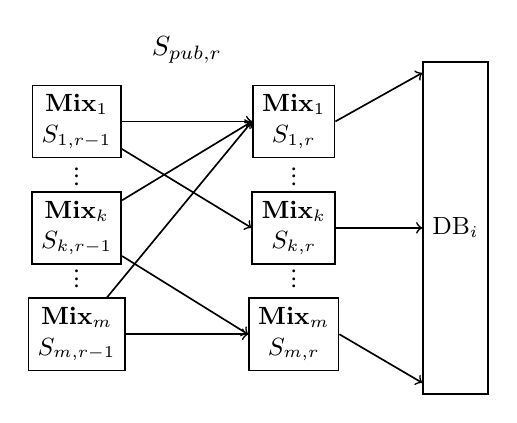
\begin{tikzpicture}[->,
auto,
semithick, 
scale=0.5,
block/.style={draw, fill=white, rectangle, font=\small}]

\node[block, align=center]							(B)		{$\textbf{Mix}_k$ \\ $ S_{k,r}$};
\node[draw=none, fill=none]    		(X)[above of=B, yshift=-1em]		[rotate=-90]{...};
\node[draw=none, fill=none]    		(Y)[below of=B, yshift=1em]		[rotate=-90]{...};
\node[block, anchor= north, align=center]			(A)[above of=B, yshift=1em]		{$\textbf{Mix}_1$ \\ $ S_{1,r}$};
\node[block, anchor = south, align=center]			(C)[below of=B, yshift=-1em]		{$\textbf{Mix}_m$ \\ $ S_{m,r}$};

\node[block, align=center]							(B')[left of=B, xshift=-5em]		{$\textbf{Mix}_k$ \\ $ S_{k,r-1}$};
\node[draw=none, fill=none]    		(X')[above of=B', yshift=-1em]		[rotate=-90]{...};
\node[draw=none, fill=none]    		(Y')[below of=B', yshift=1em]		[rotate=-90]{...};
\node[block, anchor= north, align=center]			(A')[above of=B', yshift=1em]		{$\textbf{Mix}_1$ \\ $ S_{1,r-1}$};
\node[block, anchor = south, align=center]			(C')[below of=B', yshift=-1em]		{$\textbf{Mix}_m$ \\ $ S_{m,r-1}$};


\node[block, anchor = east, minimum height=12em]		(1)[right of=B, xshift = 3em]		{$\text{DB}_{i}$};


\path[->, midway]
 (A')		edge node[above,yshift=4ex]		{$S_{pub,r}$} 	(A.west)
 (A')		edge node		{} 					(B.west)
 (B')		edge node		{} 					(C.west)
 (B') 		edge node		{} 					(A.west)
 (C') 		edge node		{} 					(A.west)
 (C') 		edge node		{} 					(C.west)

 (A.east) edge node[sloped, above]	{} 	([yshift=-2ex]1.north west)
 (B.east) edge node[sloped, above]	{} 	(1)
 (C.east) edge node[sloped, above]	{} 	([yshift=2ex]1.south west);
 
\end{tikzpicture}
\centering
\caption*{Last rounds of wrapping} \label{fig:WAS}
\end{minipage}
\hfill
\begin{minipage}[c]{0.475\textwidth}
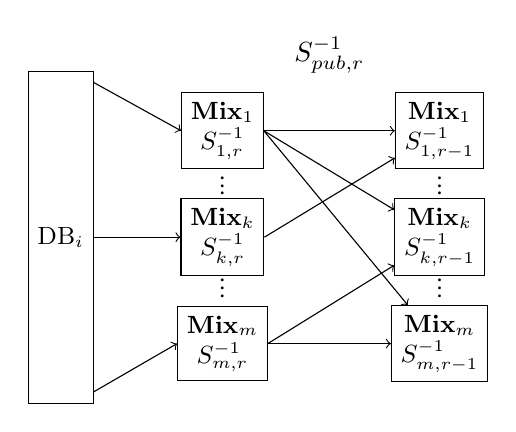
\begin{tikzpicture}[->,
auto,
thin, 
scale=0.5,
block/.style={draw, fill=white, rectangle, font=\small}]


\node[block, anchor = west, minimum height=12em] 		(0)		{$\text{DB}_i$};

\node[block, align=center]							(B)[right of=0, xshift=3em]		{$\textbf{Mix}_k$ \\ $ S_{k,r}^{-1}$};
\node[draw=none, fill=none]    		(X)[above of=B, yshift=-1em]		[rotate=-90]{...};
\node[draw=none, fill=none]    		(Y)[below of=B, yshift=1em]		[rotate=-90]{...};
\node[block, anchor= north, align=center]			(A)[above of=B, yshift=1em]		{$\textbf{Mix}_1$ \\ $ S_{1,r}^{-1}$};
\node[block, anchor = south, align=center]			(C)[below of=B, yshift=-1em]		{$\textbf{Mix}_m$ \\ $ S_{m,r}^{-1}$};

\node[block, align=center]							(B')[right of=B, xshift=5em]		{$\textbf{Mix}_k$ \\ $ S_{k,r-1}^{-1}$};
\node[draw=none, fill=none]    		(X')[above of=B', yshift=-1em]	[rotate=-90]{...};
\node[draw=none, fill=none]    		(Y')[below of=B', yshift=1em]	[rotate=-90]{...};
\node[block, anchor= north, align=center]			(A')[above of=B', yshift=1em]	{$\textbf{Mix}_1$ \\ $ S_{1,r-1}^{-1}$};
\node[block, anchor = south, align=center]			(C')[below of=B', yshift=-1em]	{$\textbf{Mix}_m$ \\ $ S_{m,r-1}^{-1}$};


\path[->, midway]
 ([yshift=-2ex]0.north east) edge node[sloped, above]{} (A.west)
 (0) edge node[sloped, above]{} (B.west)
 ([yshift=2ex]0.south east) edge node[sloped, above]{} (C.west)

 (A.east) edge node[above,yshift=4ex]	{$S_{pub,r}^{-1}$} 	(A')
 (A.east) edge node						{} 					(B')
 (A.east) edge node						{} 					(C')
 (B.east) edge node						{} 					(A')
 (C.east) edge node						{} 					(B')
 (C.east) edge node						{} 					(C');
 
\end{tikzpicture}
\centering
\caption*{First rounds of unwrapping} \label{fig:UAS}
\end{minipage}
\centering
\caption{Wrapping and corresponding unwrapping.}\label{fig:Par}
\end{figure*} 

\noindent\textbf{Using AES-CBC.} In this case, the mixes keep encrypting the records with the appended IVs during $r$ rounds of wrapping and unwrapping.\\

\noindent\textbf{Message Format.}
The client only need to send to each mix the signed message containing session keys to access the database $(id,\ token)$, information to compute which records it has been attributed $(index,\ range)$, the client's secret used to compute the shared secret $(\alpha_i,\ \alpha_i',\ \alpha_{pub},\ \alpha_{pub}')$, the number of rounds $r$, and the signed ordered $(ports,\ ips)$ of the mixes participating in the eviction.
The message format is then : $$E_{pub,\ mix_i}\left (id,\ token,\ index,\ range,\ \alpha_i,\ \alpha_i',\ \alpha_{pub},\ \alpha_{pub}',\ r,\ (port	s,\ ips)_{signed}\right )$$

\noindent\textbf{Costs.} For 128-bit security, group elements can be expressed in just 32 bytes, we have thus a maximum message size of $|addr|+XXX + 3 \cdot 8 \cdot 32 + XXX$. We have $c_{cmp} = 2\cdot r \cdot n \cdot c_{CBC}$, $c_{client}= x$, $c_{mix}= 2\cdot r \cdot n$ and $c_{com} = 2 \cdot r \cdot n+ c_{client}$.\\

\noindent\textbf{Using AES-CTR.}
When performing an eviction, the client assigns to each mix  $k=\frac{n}{m}$ distinct indexes together with a list of shared secrets from which will be derive public and private permutation seeds and encryption keys.\\
At first, the mixes fetch their allocated records from the database. They then unwrap the previous permutation: the last wrapping permutations are undone in reverse order thanks to the old private seeds and the records are decrypted with the old encryption keys before being distributed to all mixes according to the inverse permutation of the old public seeds. Then starts the wrapping, where the records are permuted according to the new seeds, encrypted with the new encryption keys and distributed to the mixes according to the new public seeds. Between the wrapping and unwrapping phases, the mixes exchanged in a cascade fashion their records and encrypt them with both the new and old key.\\

\noindent\textbf{Message Format.}
The client send the same data as in the AES-CBC case. The message format is then : $$E_{pub,\ mix_i}\left (id,\ token,\ index,\ range,\ \alpha_i,\ \alpha_i',\ \alpha_{pub},\ \alpha_{pub}',\ r,\ (ports,\ ips)_{signed}\right )$$

\noindent\textbf{Costs.} For 128-bit security, group elements can be expressed in just 32 bytes, we have thus a maximum message size of $|addr|+XXX + 3 \cdot 8 \cdot 32 + XXX$. We have $c_{cmp} = 2\cdot (r+m) \cdot c_{CTR} $, $c_{client}=x$, $c_{mix}= (2r+m)\cdot n$. The total communication cost is $c_{com}= (2r+m)\cdot n + c_{client}$.

\section{Security Proof}\label{Security}

We first remark that all of the eviction metadata is independent of data content, it is entirely determined by the sole parameter $n$ and is the same for any access. The data content is also never revealed to the adversary and is refreshed upon reception by every mix.
We argue that the adversary can win the game in only two ways: decrypting the records or finding out the record order before eviction. 

\subsection{In Search of the Lost Order.}
The client has sent to each mix private, and potentially public, group elements chosen as random from which the permutation keys are retrieved. The randomness of the seeds was increased thanks to the use of a key derivation function.\\

\noindent\textbf{Cascade mixnet.}
In this architecture, the whole database is sent from a mix to another. To know the index of any block, the adversary needs to retrieve the group elements sent to the uncompromised mixes. \\

\noindent\textbf{Parallel mixnet.}
In this architecture, chunks of the database are exchanged between mixes. The adversary can benefit of it as some records may never go to uncompromised mixes.\\
Goodrich in 2012 ~\cite{goodrich2012anonymous}, proved the security of such scheme using the sum of squares metric. If we note by $p(i,t)$ the probability the adversary thinks that the a particular card is at index $i$ at round $t$, $m-m_a$ the number of uncorrupted server(s) and by $\Phi(t)= \sum_{i}^{n}\left (p(i,t) - 1/n \right)^2$ the sum of squares metric, we have that $$E[\Phi(t)] = \left (1 - (m-m_a) \cdot \frac{k-1}{n-1}\right )^{t}$$\\
To have $\Phi(t) \leq n^{-c}$ with $m-m_a=1$, we need $cm \log n \leq r \leq 2cm \log(n)$, the upper bound being the value we propose in Section~\ref{kRTS}. The value we propose in Theorem~\ref{sec:kOM}, $\frac{m}{2} \cdot log\left ( \frac{n}{s} \right )$, accounts for the indistinguishability assumption we made: we do not want to hide the position of every record, only the position of $s$ of them (the accessed ones). ?

\subsection{In Search of the Lost Key.}
We assume here the adversary knows the invariant position of some of the records he asked the user to query. 

\noindent\textbf{The CBC case.}
In the CBC case, the blocks and IVs are encrypted again and again with AES in CBC mode. If a block was accessed, it is however encrypted only once by the user before the eviction.\\

\noindent\textbf{The CTR case.}
In the case of CTR, the adversary only needs to discover the uncompromised mixes' bindings. 

uncompromised mix blindings are never known by the adversary as the records are encrypted with AES-CTR when being (un)blinded. Thereby, the records after the unwrapping are undistinguishable from random arrays, and the adversary cannot see which records were accessed.

\section{Evaluation}\label{Evaluation}
\subsection{Implementation and Benchmark}\label{Implementation}
\subsection{Performances}\label{Performance}
performance per enc, performance per design, performance with implementation
\subsection{Comparison}\label{Comparison}
Comparison of CBC and tagging

\begin{table*}
\begin{minipage}[t][][b]{.475\textwidth}
\vspace{0pt}
\centering
\begin{tabular}{*4c}
\toprule
    				& $C_{comp}$  	 & $C_{comm}$		& $C_{access}$\\
\midrule
Cascade - CBC   &  17.5 		& 19.1   		& 17.5  \\
Cascade - CTR   &  11.8 		& 12.7   		& 29.3  \\
Parallel - CBC  &  6.6  		&  5.6   		& 35.9  \\
Parallel - CTR  &  6.6  		&  5.6   		& 35.9  \\
\bottomrule
\end{tabular}
\centering
\caption{Cost comparison of designs.}
\end{minipage}
\hfill
\begin{minipage}[t][][b]{.475\textwidth}
\vspace{0pt}
\begin{tabular}{*4c}
\toprule
    				& $m=3$  	 & $m=5$		& $m=7$\\
\midrule
Cascade - CBC   &  17.5 		& 19.1   		& 17.5  \\
Cascade - CTR   &  11.8 		& 12.7   		& 29.3  \\
Parallel - CBC  &  6.6  		&  5.6   		& 35.9  \\
Parallel - CTR  &  6.6  		&  5.6   		& 35.9  \\
\bottomrule
\end{tabular}
\centering
\caption{Time comparison of designs,\\with $n=\frac{1024^3}{4\cdot 1024}$, $s=\sqrt n$.}
\end{minipage}
\end{table*}


\section{Discussion}\label{Discussion}

\subsection{Active Adversary}\label{Active Adversary}
As misbehaving mixes are already discarded in the eviction setup, we could integrate in the client a light-weight local mix reputation system.
Randomized Partial Checking


\subsection{Differentially Private Oblivious Shuffle}\label{DPOS}
We could ask the mixes to process only a fraction of rounds $r \approx \frac{n}{2\cdot k }  \cdot \log \left (\frac{n}{s}-0.5 \right)$ to increase even more the efficiency of the eviction.

In the worst case scenario where an adversary $\mathcal{A}$ controls all but one mixes, the probability  $\mathcal{A}$ knows where a record is at the end of the eviction is $\delta= \Pr \left ( \mathcal{A} \text{ knows a record index}\right ) = \left ( 1 - \frac{1}{m} \right )^r$ where is $r$ the number of rounds.

To prevent such case, we can make each mix permute every allocated sections of the database and then begins the Oblivious Merge. We would thus add $2 \cdot m^2$ permutations for the whole eviction....

\section{Acknowledgement}
Danezis was supported by H2020  PANORAMIX Grant (ref. 653497) and EPSRC Grant EP/M013286/1; and Toledo by Microsoft Research.


\section{Conclusion}\label{Conclusion}
\begin{itemize}
 \item New ORAM with mix-net
 \item amortizable eviction
 \item can fetch while eviction running
 \item multi-user friendly as all the secrets are on the server
\end{itemize}

\bibliography{mix_oram}
\bibliographystyle{splncs03}

\section{Appendix}
\subsection{Proof $k$-RTS}\label{proof:kRTS}
\begin{proof}
To first prove the upper bound and variance, we use Diaconis et al. results~\cite{aldous1986shuffling} which states that $\tau$ defined in the following game is a strong stationary time.
In a random transposition shuffle, the cards chosen by the right and left hands at time $t$ are respectively called $R_t$ and $L_t$. Assuming that when $t=0$, no card is marked, we mark $R_t$ if
$R_t$ was unmarked before and either $L_t$ is marked or $L_t = R_t$. The variable $\tau$ represents the time when every card has been marked, we call it the stopping time.

Let be $\tau_t$ the number of transpositions after the $t^{th}$ card is marked, up to and including when the $(t+1)^{th}$ is marked. $$\tau = \sum_{i=0}^{n-1} \tau_i$$
The $\tau_t$ are independent geometric variables with probability of success $p_t$ as implied by the game rules.
The probability of success corresponds to the probability of marking at least one card, one to $t$ cards exactly. To do so, the right cards must be chosen from the unmarked set, comprising $n-t$ cards at time $t$,
and the left cards from the union of the marked set and the right cards.
\begin{align*}
 p_t &= \sum_{i=1}^{min(k,n-t)} {k \choose i} \cdot {t+1 \choose i} \cdot {n-t \choose i}\cdot{n \choose i}^{-2}&\\
 &= \frac{1}{n^2} \cdot \left ( k \cdot (t+1)\cdot(n-t) + \alpha_{n,t,k}\right ),\ 0 < \alpha_{n,t,k} = \mathcal{O}\left(n^{-k}\right )
\end{align*}

We can thus rewrite $\tau$'s expectation as following.
\begin{align*}
 E(\tau) &= \sum_{t=0}^{n-1} \frac{1}{p_{t}} = \sum_{t=0}^{n-1} \frac{n^2}{k \cdot (t+1)\cdot(n-t) + \alpha_{n,t,k}}&\\
 &< \sum_{t=0}^{n-1} \frac{n^2}{k \cdot (t+1)\cdot(n-t)}  &\\
 &< \frac{1}{k} \cdot \frac{n^2}{n+1} \cdot  \sum_{t=0}^{n-1} \left ( \frac{1}{t+1} + \frac{1}{n-t} \right ) &\\
% &< \frac{2}{k} \cdot \frac{n^2}{n+1} \cdot H_n  \\
 &< \frac{2}{k} \cdot \frac{n^2}{n+1} \cdot \left( \ln(n) + \gamma +\mathcal{O}(\frac{1}{n}) \right), \gamma = \lim_{n \to \infty} H_n - \ln(n)& \\
 \end{align*}
 \begin{align*}
 var(\tau) &= \sum_{t=0}^{n-1}\frac{1-p_t}{{p_t}^2}\ <\  \sum_{t=0}^{n-1}\frac{1}{{p_t}^2} &\\
 &< \sum_{t=0}^{n-1}\frac{1}{\left ( k \frac{(t+1)\cdot(n-t)}{n^2} + \alpha_{n,t,k}\right )^2}\\\
 &<\ \sum_{t=0}^{n-1} \frac{1 }{\left ( k \frac{(t+1)\cdot(n-t)}{n^2} \right )^2} &\\
 %&< \frac{n^4}{k^2} \left ( \sum_{t=0}^{\frac{n}{2}-1} \frac{1}{\left ( (t+1)(n-t)\right )^2}  + \sum_{t=\frac{n}{2}}^{n-1} \frac{1}{\left ( (t+1)(n-t)\right )^2} \right ) &\\
 &< 2 \cdot \left (\frac{n}{k} \right )^2 \cdot \left (\frac{n}{n/2} \right )^2 \cdot \sum_{t=0}^{n/2-1} \frac{1}{(t+1)^2} &\\
 &< \frac{4}{3} \pi^2 \cdot \left (\frac{n}{k} \right )^2 
\end{align*}
\\

To now prove the lower bound of $\tau$, we will compare the number of fixed points of a permutation $\sigma$, $F(\sigma)$, for our shuffle, the permutation
obtained from the identity by applying $kt$ random transpositions $ P^{kt}(id, \cdot)$, and the uniform distribution $\pi$, or more precisely compare the corresponding probabilities over the set $A=\{\sigma : F(\sigma) \geq \frac{\mu}{2} \}$.
We can say that after $t$ shuffles, the number of untouched cards of our shuffle has the same distribution as the number $R_{2kt}$ of uncollected coupon types after $2kt$ steps of a coupon collector chain
and that about $ P^{kt}(id, \cdot)$ that the associate $F(\sigma)$ is at least as large as the number of cards that were touched by none of the transpositions, i.e. $P^{kt}(id,A) \geq P(R_{kt}\geq A) $.

We know that the $R_{2kt}$ has expectation $\mu = np$  with $p=\left ( 1 - \frac{1}{n} \right )^{2kt}$, variance $var = np(1-p) <\mu$ and by Chebyshev, we know that $\Pr(R_{2kt}\leq \frac{\mu}{2})\leq \frac{4}{\mu}$
as $\Pr(|R_{2kt} - \mu|\geq \frac{\mu}{2}) = \Pr(R_{2kt} \geq \frac{3\mu}{2}) + \Pr(R_{2kt} \leq \frac{\mu}{2}) > \Pr(R_{2kt} \leq \frac{\mu}{2})$.\\

By Markov's inequality we know that $\pi(A) \leq \frac{2}{\mu}$.\\

As $P^{kt}(id,A) \geq P(R_{kt}\geq A) $, we also have $P^{kt}(id,A^c) \leq P(R_{2kt}\leq A) \leq \frac{4}{\mu} $ which leads to $P^{kt}(id,A)\geq1 - \frac{4}{\mu}$.\\

Thus we have $d(t)=||P^{kt}(id,) - \pi ||_{TV} \geq |1 - \frac{4}{\mu} - \frac{2}{\mu}| \geq 1 - \frac{6}{\mu}$.\\

We want to find the minimum $t$ such that $1-\frac{6}{\mu}\geq \epsilon$, which is equivalent to $n \cdot \left ( 1 - \frac{1}{n} \right )^{2kt} \geq \frac{6}{1-\epsilon}$ and to
$$\log\left(\frac{n\cdot (1-\epsilon)}{6}\right) \geq 2\cdot k\cdot t \cdot \log \left ( \frac{n}{n-1} \right )$$
As $\log(1+x) \leq x$, the previous inequality holds if $\log\left(\frac{n\cdot (1-\epsilon)}{6}\right) \geq   \frac{2kt}{n-1} $ which means that if $t\leq \frac{n-1}{2k}\cdot \log\left ( \frac{n(1-\epsilon)}{6}\right )$ then $d(t)\geq \epsilon$.
Thus,
$$\tau \left (\epsilon \right ) \geq \frac{n-1}{2k} \ln(n\cdot \frac{1-\epsilon}{6}) $$.
\end{proof}

\subsection{Proof of Oblivious Merge}\label{proof:OM}
\begin{proof}
We want to find the mixing time $\tau(\epsilon)$ of our oblivious merge of two sets of indistinguishable elements. To do so, we use the bound of the mixing time of an irreducible ergodic Markov Chain, where $p = \frac{1}{|V|}$ and $1-\lambda^*$ is the spectral gap,
$$\frac{\lambda^*}{1-\lambda^*} \cdot \log\left(\frac{1}{2 \epsilon} \right)\leq \tau(\epsilon) \leq \frac{1}{1-\lambda^*}\cdot \log \left( \frac{1}{2 \epsilon \cdot \sqrt{p}}\right) $$

We now want to find a bound for $\lambda^*$. We represent the arranging of merge of the 2 distinct sets by the graph $\mathcal{G}$, a $k$-regular graph with $v$ vertices corresponding to the different orderings and the undirected edges to transpositions of two elements.
By definition, the eigenvalues of the transition matrix of the $\mathcal{G}$ are $k={\lambda'}_0 > {\lambda'}_1 \geq  ... \geq {\lambda'}_{n-1}$, and we have,
$$\text{diam}\left( \mathcal{G}\right) \leq \frac{log(v-1)}{log(\frac{k}{{\lambda'}^*})}+1 \text{ with } {\lambda'}^* = max_{i\neq0}({\lambda'}_i)= k \cdot \lambda^*$$
with $diam\left( \mathcal{G} \right)=s$ the diameter of the graph, $v= {n \choose s}$ the number of vertices and $k=s\cdot(n-s)$.\\


We can thus find a first relation:
\begin{align*}
log(\frac{k}{{\lambda'}^*}) &= log(\frac{1}{{\lambda}^*}) \leq\frac{\log(v-1)}{\text{diam}\left(\mathcal{G}\right)-1}&\\
log({{\lambda}^*}) &\geq  \frac{log(v-1)}{1-\text{diam}\left(\mathcal{G}\right)}&\\
{\lambda}^* &\geq (v-1)^{\frac{-1}{\text{diam}\left(\mathcal{G}\right)-1}}\\
{\lambda}^* &\geq \left ({n \choose s}-1 \right )^{\frac{1}{1-s}} \geq \left (\frac{n\cdot e}{s} \right )^{\frac{s}{1-s}}
\end{align*}

And can derive the minimum value of $\Delta=\frac{\lambda^*}{1-\lambda^*}$,
\begin{align*}
 \Delta &= \frac{1}{\left (\lambda^*\right )^{-1}-1}\\
 &\geq \frac{1}{\left (\frac{n \cdot e }{s} \right )^{\frac{s}{s-1}}-1}\\
\end{align*}


To find an upper-bound of $\lambda^*$, we will focus on the spectral gap bounding.
Let's $\mathcal{G}_{0,1}=\{0,1\}^n$ be the group of elements with the XOR operation and $\mathcal{S}=\{x \in \mathcal{G},\ weight(x)=s\}$ the symmetric subset of $\mathcal{G}$ of n-binary array with $s$ 1s and $n-s$ 0s.
We call $Cay_{n,s}=Graph\left(  \mathcal{G}_{0,1}, \mathcal{S} \right) $ the Cayley graph generated from these structures.

\begin{lemma}
Let $\mathcal{G}$ be a finite Abelian group, $\chi\ :\  \mathcal{G} \rightarrow \mathbb{C}$ be a character of $\mathcal{G}$, $\mathcal{S} \subseteq \mathcal{G}$ be a symmetric set.
Let $M$ be the normalized adjacency matrix of the Cayley graph $G = Cay(\mathcal{G},\mathcal{S})$.
Consider the vector $x \in \mathbb{C}^\mathcal{G}$ such that $x_a = \chi(a)$. Then x is an eigenvector of $G$, with eigenvalue $$ \frac{1}{\mathcal{S}} \sum_{s\in \mathcal{S}} \chi\left(s\right)$$
\end{lemma}

\begin{theorem}
The Cayley graph $Cay_{n,s}$ has for eigenvalues $\mu_0 = 1 > \mu_1 \geq ... \geq \mu_n$ with, 
$$\mu_r = \frac{1}{\left | \mathcal{S} \right |} \sum_{i=1}^{min(r, n-r)} \left ( -1 \right )^i {r \choose i}{n-r \choose s-i}\\$$
\end{theorem}

\begin{subproof}
$\forall r \in \{0,1\}^n$, with $\chi_r(x)=\left ( -1 \right )^{\sum r_i \cdot x_i}$, we have,
\begin{align*}
\mu_r &= \frac{1}{\mathcal{S}} \sum_{s\in \mathcal{S}} \chi\left(s\right) \\
&= \frac{1}{\left | \mathcal{S} \right |} \sum_{s\in \mathcal{S}} \left ( -1 \right )^{\sum r_i \cdot s_i} \\
&=  \frac{1}{\left | \mathcal{S} \right |} \left ( \left | ``1" \right | - \left | ``-1"  \right| \right ) \\
&= \frac{1}{\left | \mathcal{S} \right |} \sum_{i=1}^{min(r, s)} \left ( -1 \right )^i {r \choose i}{n-r \choose s-i} \\
&= 1 - \frac{2}{{n \choose s}} \cdot \sum_{i=0}^{min(\frac{r-1}{2}, \frac{s-1}{2})} {r \choose 1+2i}{n-r \choose s-2i-1} \\
&= \frac{{n-r \choose s}}{{n \choose s}} \ _2F_1(-r,-s,n-2r+1,-1)
%&= \frac{1}{\left | \mathcal{S} \right |} \left [ \sum_{i=0}^{min(\frac{r}{2},\frac{n-r}{2})} {r \choose 2i}{n-r \choose s-2i} - \sum_{i=0}^{min(\frac{r-1}{2}, \frac{n-r-1}{2})} {r \choose 1+2i}{n-r \choose s-2i-1}\right] 
\end{align*}
\end{subproof}


Remark. We recognize here the Vandermonde identity with alternating numbers. We argue that the eigenvalues of the Cayley graph $Cay_{n,s}$ are all positive as the smallest eigenvalue is null.
For $r=n-r$, the expression simplifies to $\mu_r = {r \choose \frac{n}{2}}$ if $n$ even, 0 otherwise.
For $r=1$, the expression simplifies to $\mu_1 = 1 - 2\cdot \frac{s}{n}$, the spectral gap of $Cay_{n,s}$ is thus equal to $2\cdot \frac{s}{n}$.\\\

We notice that the first graph $\mathcal{G}$ actually is a sub-graph of $Cay_{n,s}$ and as such the the adjacent matrix of the first graph is included in the second's.
For $s>1$, $Cay_{n,s}$ is divided in two sub-graphs representing the cosets of $\{0,1\}^n$ as $\mathcal{S}$ is not a generating group of $\mathcal{G}_{0,1}$, $\mathcal{G}$ is only contained in one of the sub-graphs.
We use the Cauchy's Interlace Theorem to bound the eigenvalues of $\mathcal{G}$ with the ones of $Cay_{n,s}$,.

\begin{theorem}
Let $M$ be a Hermitian $n \times n$ matrix with eigenvalues ${\mu'}_0\geq ... \geq {\mu'}_{n-1}$ and $N$ a $m \times m$ sub-matrix of $M$ with eigenvalues ${\lambda'}_0\geq ... \geq {\lambda'}_{m-1}$ , we have
$$ {\mu'}_i \geq {\lambda'}_i \geq {\mu'}_{n-m+i+1} $$
\end{theorem}

We are here only interested in an upper-bound of $\lambda*$, as we have $\mu_{2^n+2-{n \choose s}}\leq \lambda_1\leq 1-2\frac{s}{n}$ and $0 \leq \lambda_n \leq \mu_2$, $\lambda* \leq 1-2\frac{s}{n}$. We thus have $\frac{1}{1-\lambda*}\leq\frac{n}{2\cdot s}$
\end{proof}

\subsection{Proof of Fake access}
\begin{proof}
 We want to prove that the average number of fake access is 0 in case of a uniform distribution. To do so, we consider the Markov chain and its Transition Matrix.
 The transition matrix $P$ represents the $s$ transient state, in which the stash is not completely filled, and the absorption state in which the stash is full.
Thus, $P$ can be decomposed in 4 sub-matrices: the square sub-matrix $Q_s$ representing all the transient state, the column matrix R with the probabilities of transitioning to the absorbing state, the null row matrix and the absorption matrix.
\[
\begin{bmatrix}
   Q_s & R \\
   0_{1\times s}   & I_1 \\
\end{bmatrix}
\]
To find the average number of steps from one state to the absorbing one, we have solve the following equation, each row corresponding to the average number of steps from the corresponding state (the stashed filled with some records) to the state where the stash is full.
\begin{align*}
 t &= \left (\sum_{k=0}^{\infty} {Q_s}^k \right ) 1 \\
   &= (I_s -Q_s )^{-1} 1
\end{align*}
This equation has a solution since $M=I_s -Q_s$ have independent rows and thus an inverse that we call $N$.
By calculus we find that,
\begin{align*}
 n_{i,j} &= 0 &\text{ if } i>j,\\ 
 n_{i,j} &= \frac{1}{m_{i,i}} &\text{ if } i=j,\\
 n_{i,j} &= - n_{i+1,j } \cdot \frac{m_{i,i+1}}{m_{i,i}} &\text{ if } i<j 
\end{align*}
which can be simplified by
\begin{align*}
 n_{i,j} &= 0 &\text{ if } i>j,\\ 
 n_{i,j} &= \frac{1}{m_{j,j}} \prod_{k=1}^{j-1} \left ( - \frac{m_{i,k+1}}{m_{k,k}}\right ) &\text{ if } i\leq j
\end{align*}
We only want to calculate the first solution $S_1$ from the equation.
\begin{align*}
 S_1 &= \sum_{j=0}^{s-1} \frac{1}{m_{j,j}} \prod_{k=1}^{j-1} \left ( - \frac{m_{i,k+1}}{m_{k,k}}\right ) \\
     &= \sum_{j=1}^{s-1} \frac{1}{m_{j,j}} \text{ as } m_{i,k+1}= -m_{k,k} \\
     &= \sum_{j=0}^{s-1} \frac{1}{1-\frac{j}{n}} = \sum_{j=0}^{s-1} \left (1 + \frac{j}{n-j} \right ) \\
     &= s + \sum_{j=0}^{s-1} \frac{j}{n-j} \\   
\end{align*}
As $s$ steps are required to fill the stash, we thus find the following inequality for the number of fake access $f$:
$$ \frac{s \cdot (s+1)}{2 \cdot n} < f < \frac{s \cdot (s+1)}{2 \cdot (n+1-s)} $$
\end{proof}
\end{document}
